\section{System Analysis and Design}
\label{analysis}

For this year's contest, we opted for developing a new team using the \jacamo~\cite{boissier:2011} platform instead of just improving the last year team. The programming model of \jacamo\ provides high-level support for developing MAS considering agents, environment, and organization as \emph{first-class} entities. The development of these three dimensions is based on three different technologies: Jason \cite{bordini:2007}, for programming the agents; \cartago \cite{ricci:2011}, for programming the environment; and \moise \cite{hubner:2007} for programming the organization. Thus, this year the organization and environment, which were previously implemented as part of the agent code, have now been programmed with proper organizational and environmental elements according to the aforementioned models and technologies.

\subsection{Organizational Dimension}

As \jacamo supports organizational programming, part of the coordination of team agents is modeled in the organizational dimension instead of being modeled as skills of the agents. The organization provides guidelines for the achievement of the overall system goals, but the agents remain autonomous to decide how to achieve them. For example, the organization informs that an agent is obligated to probe the vertices, but the agent is autonomous about ``how'' to do it, based on its local knowledge about the world. However, the autonomy can be constrained by means of organizational norms.

Fig.~\ref{fig:org_ss} shows the structural specification (SS) of the team using the \moise\ notation. Notice that the SS is designed based on the roles of the contest scenario. The team is divided into two \emph{sub-teams}. Besides, the team has three minor subgroups: \emph{special operations}, \emph{special exploration}, and \emph{pivots}. An agent can play more than one role at the same time. For example, an \emph{explorer} can also play \emph{explorer leader} and \emph{special explorer} roles. One agent plays the role \emph{leader} and is responsible to manage the overall organization (e.g. designating the roles of the other agents). The functional specification (FS) (Fig.~\ref{fig:org_fs})) specifies the goals (i.e. specific states of affairs) that the agents must achieve and distributes these goals to the agents (by means of missions). The overall goal (\emph{domain mars}) consists in a decomposition tree where the leaves are the goals that can be achieved by the agents. The goals are grouped in four \emph{missions} ($m1$, $m2$, $m3$, and $m4$). Finally, the normative specification (NS) (Fig.~\ref{fig:org_ns}) relates roles to missions. For example, as the \emph{explorer leader} is obligated to commit to mission $m4$, it is obligated to achieve the goals \emph{define initial hill}, \emph{conclude first phase}, and \emph{dismiss agent}.

\begin{figure}[th]
 \vspace{-5mm}
 \centering
 \subfigure[Structural specification]{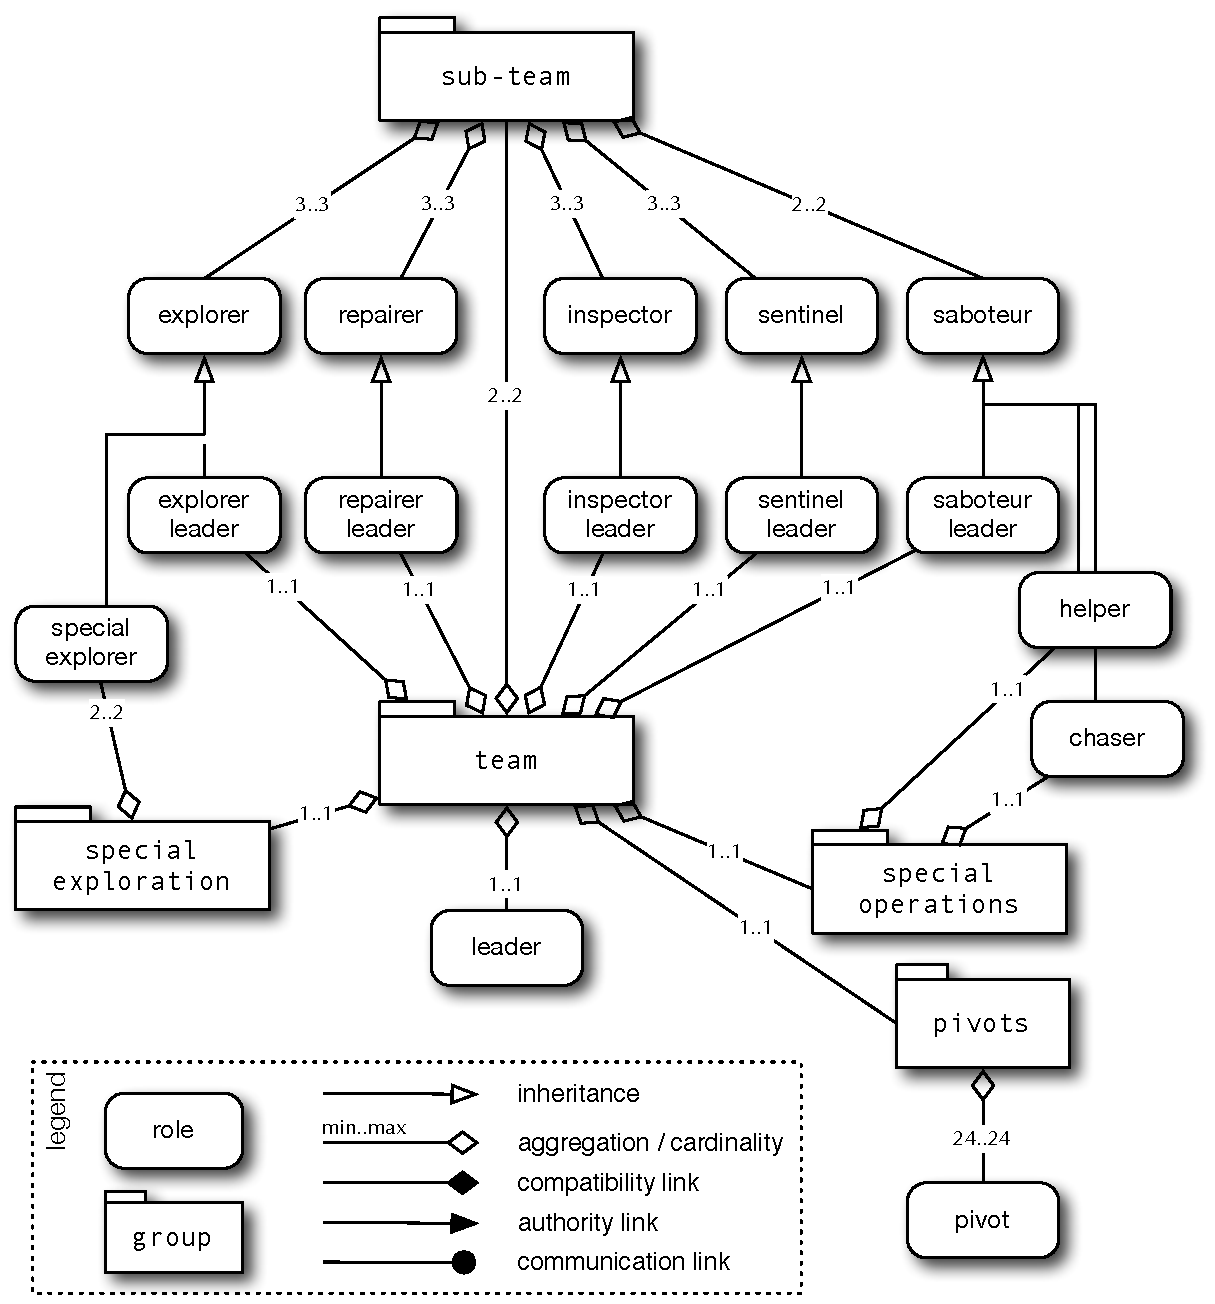
\includegraphics[width=0.54\textwidth]{figs/ss.pdf}\label{fig:org_ss}}
 \subfigure[Functional specification]{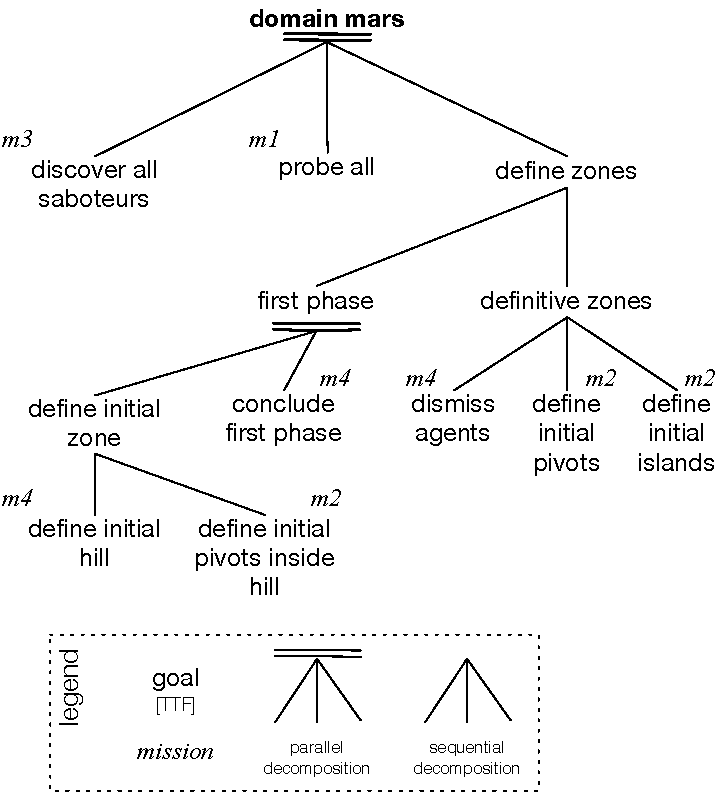
\includegraphics[width=0.45\textwidth]{figs/fs.pdf}\label{fig:org_fs}}
 \subfigure[Normative specification]{\setlength{\tabcolsep}{12pt}
\begin{tabular}{llll}
\emph{norm} & \emph{role} &   & \emph{mission}\\
\midrule
n1 & explorer & obligation & m1\\
n2 & sentinelLeader & obligation & m2\\
n3 & inspector & obligation & m3\\
n4 & explorerLeader & obligation & m4
\end{tabular}

\label{fig:org_ns}}
 \vspace{-3mm}\caption{Organizational Specification}
 \label{fig:org}
 \vspace{-3mm}
\end{figure}

Along the development of the team, we performed some experiments introducing \emph{count-as rules}~\cite{brito:2012}. Count-as rules changes in the organization as the result of facts occurring in the environment. For example, without count-as rules, a specific agent has to set up the organizational infrastructure and explicitly adopt the role of \emph{leader}. With count-as rules, it is possible to state that such setup \emph{counts-as} the adoption of the \emph{leader} role. In another example, without count-as rules, the agents have to reason about the organizational structure, checking their roles, and committing to missions according to that roles. With count-as rules, it is possible to model that playing of a specific role \emph{counts-as} the commitment to a specific mission. The use of count-as rules simplifies the reasoning and action of the agents, as they do not need to perform some actions on the organization (e.g. they do not need to reason and to act to commit to missions). Besides, count-as rules contribute to keep the organization in a consistent state as some organizational actions do not depend on the agents actions. Due to time constraints, the count-as rules were not added to the tournament team. However, the experiments indicate that the rules seem a suitable approach for further versions of the team.

\subsection{Environment Dimension}\label{sec:env}

The environment for our agents has two parts. The first part provides integration with the contest simulation by means of EISMASSim framework~\cite{behrens:2011} and is well defined in the contest documentation. The second part is provided by \jacamo\ artifacts that agents perceive and use to achieve their goals. In our team, the information about the inspected enemies is managed by an artifact.  We also conceived an artifact responsible to manage all the graph structure. However, since we used the same graph structure and algorithms of the last year, which were based on Java shared memory, we decided to not move this previous implementation into a specific \cartago\ artifact because it would require more time. Therefore, part of the environment is developed in \cartago\ and another part was kept in ``pure Java'', accessed by means of Jason internal actions, as we did last year. It is a future work to unify all perceptions and actions under the \cartago\ approach.


\subsection{Agent Dimension}

The agents may behave proactively or reactively, in accordance with the needs. For example, a damaged agent will proactively call a repairer and all agents promptly react to the environment events, like the start of a new  simulation step. 

Agents share information by two mechanisms: messages and blackboards. Since it was not so appropriate to broadcast everything between the agents because we would have $28 \times 27$ messages\footnote{The team is composed of 28 agents.}, we chose to send messages about few things. For example, when agents are disabled, they call a repairer; when enemies invade some team area, the saboteurs are notified; and when some vertex is probed, the explorers broadcast the value of the vertex. Some information is also important to exchange between agents of the same kind to avoid them performing the same action. For example, when there are two saboteurs with enemies in the same vertex, they need to communicate to decide which enemy each one will attack. We used the same solution for explorers and repairers to avoid repairing the same agent and to avoid probing the same vertex. Messages are also used to inform agents about the zones they should help to conquer.

The second (indirect) communication mechanism is the use of blackboards and artifacts as commented on Sec.~\ref{sec:env}. In this case, the agents share the graph structure, the information about the inspected agents, and the position of the enemies and team mates. Finally, the remaining data, such as their own health, energy, zone scores, or visible vertices, is private for each agent.

We defined a priority among the agents to avoid conflicting actions (like two agents probing the same vertice). The agent with the highest priority chooses its action first and informs the others of the same role about its decision. Then the agent with the second highest priority does the same and so forth.\footnote{Notice that sharing the information about the chosen action is not enough to solve the problem. Some coordination is required to efficiently solve it. Although this coordination is an organizational issue, this priority solution was coded in the agent dimension and it remains as a future work to model it in the organizational dimension.} However, actions like survey and inspect do not follow this priority approach. That means two agents can inspect or survey at the same target to try to guarantee some of them will be successful. 
%TODO: For instance, an agent chooses the action ``a'', another agent chooses the same, they then share these decisions, discover the conflict, both change their decision possibly for another identical action, announce, ...   eu tirarei essa parte...
\subsection{Testing}

To develop the team we used a particular incremental process. We performed weekly meetings to define the team strategies. These strategies were implemented and tested during the week and, in the next meeting, these results were considered to define new improvements. To evaluate the team strategies and ensure the competitiveness, we tested our team by simulating a great amount (more than 1000) of matches against our 2012 team~\cite{smadas:2012}, the 2012 Python-DTU team, and previous versions of our current team. The aim of the tests was to evaluate the overall performance of the team in different maps, adopting different strategies and facing different strategies from the opponent. In addition, we participated in all test matches during the testing phase to evaluate the connection and a couple of strategies.
